% Run
% xelatex "\def\ishandout{1} \input{../lecture-header}

\LuaCodeDebugOn
\luaexec{dofile("src/tree.lua")}

\begin{document}

\title{Árvores Binárias}

\frame{\maketitle}

\begin{frame}{Árvores binárias}

Uma *árvore binária T* é um conjunto finito de elementos
denominados nós ou vértices, tal que:

- $T\in\emptyset$ e a árvore é dita vazia;
- Existe um nós especial $r$, chamado {\it raiz\/} de $T$, e os
restantes podem ser divididos em dois subconjuntos disjuntos, $T^E_r$
e $T^D_r$, a {\it subárvore esquerda\/} e a {\it direita} de $r$, as
quais são também árvores binárias.

\end{frame}

\begin{frame}{Árvore estritamente binária}

\begin{columns}
\begin{column}{.5\textwidth}
\footnotesize
Uma árvore {\bf estritamente binária} é
uma árvore binária em que cada nó possui
$0$ ou $2$ filhos.
\end{column}

\begin{column}{.5\textwidth}
    \begin{tikzpicture}
\tikzset{T/.style={circle,draw},
sibling angle=60}

\def\shift{1cm}

\node[T] (root) {} []
      child {node[T] [xshift=-.5*\shift] {}}
      child {node[T] [xshift=.5*\shift] {}
             child {node[T] [xshift=-.25*\shift] {}
                    child {node[T][xshift=-.25*\shift] {}}
                    child {node[T][xshift=-.25*\shift] {}}}
             child {node[T] [xshift=.25*\shift] {}}
};

\end{tikzpicture}
                     
\end{column}

\end{columns}

\end{frame}

\begin{frame}{Árvore binária completa}

\begin{columns}
\begin{column}{.5\textwidth}
\scriptsize
Uma {\bf árvore binária completa} apresenta
as seguintes propriedades:
se $v$ é um nó tal que alguma subárvore de $v$ \ é
vazia, então $v$ localiza-se no último (maior) \ ou penúltimo nível da
árvore.
\end{column}

\begin{column}{.5\textwidth}
   \begin{tikzpicture}
\tikzset{T/.style={circle,draw},
sibling angle=60}

\def\shift{1cm}

\node[T] (root) {} []
      child {node[T] [xshift=-.5*\shift] {}
                  child {node[T] [xshift=-.25*\shift] {}}
                  child {node[T] [xshift=-.25*\shift] {}}}
      child {node[T] [xshift=.5*\shift] {}
             child {node[T] [xshift=-.25*\shift] {}
                    child {node[T][xshift=-.25*\shift] {}}
                    child {node[T][xshift=-.25*\shift] {}}}
             child {node[T] [xshift=.25*\shift] {}}
};


\end{tikzpicture}

\end{column}
\end{columns}

\end{frame}

\begin{frame}{Árvore binária cheia}

\scriptsize Um {\bf árvore binária cheia} apresenta as seguintes
propriedades: 
se $v$ é um nó tal que alguma subárvore de $v$ \
é vazia, então $v$ localiza-se no último \
 nível da árvore.

\begin{center}
        \begin{tikzpicture}
\tikzset{T/.style={circle,draw},
sibling angle=60}

\def\shift{3cm}

\node[T] (root) {} []
      child {node[T] [xshift=-.5*\shift] {}
                      child {node[T] [xshift=-.1*\shift] {}
                                     child {node[T] [] {}}
                                     child {node[T] [] {}}
                     }
                     child {node[T] [xshift=.1*\shift] {}
                                    child {node[T] [] {}}
                                    child {node[T] [] {}}
                     }}
      child {node[T] [xshift=.5*\shift] {}
                     child {node[T] [xshift=-.1*\shift] {}
                                    child {node[T][] {}}
                                    child {node[T][] {}}
                     }
                     child {node[T] [xshift=.1*\shift] {}
                                    child {node[T][] {}}
                                    child {node[T][] {}}
                     }
};


\end{tikzpicture}

   \end{center}

\end{frame}

\begin{frame}{Árvore binária: propriedades}

\begin{center}
        \begin{tikzpicture}
\tikzset{
        every node/.style={font=\scriptsize},
        every path/.style={draw},
        T/.style={circle,draw},
        sibling angle=60,
        L/.style={dashed} % level
}

\def\shift{3cm}

\foreach \Y/\L in {2/{$n$ -- n$^{o.}$ de nós},1.5/{$l$ -- nível},1/{$h$ -- altura}} {
         \node at (4,\Y) {\L};
}

\node at (0,2) {$n_l= 2^l = 1+ \sum_{i=0}^{l-1}2^i$};
\node at (0,1) {$n_h= 2^{h+1}-1$};

\node[T] at (0,0) (root) {} []
      child {node[T] [xshift=-.5*\shift] {}
                      child {node[T] [xshift=-.1*\shift] {}
                                     child {node[T] [] {}}
                                     child {node[T] [] {}}
                     }
                     child {node[T] [xshift=.1*\shift] {}
                                    child {node[T] [] {}}
                                    child {node[T] [] {}}
                     }}
      child {node[T] [xshift=.5*\shift] {}
                     child {node[T] [xshift=-.1*\shift] {}
                                    child {node[T][] {}}
                                    child {node[T][] {}}
                     }
                     child {node[T] [xshift=.1*\shift] {}
                                    child {node[T][] {}}
                                    child {node[T][] {}}
                     }
};

\foreach \j/\n/\y in {0/1/.2, 1/2/1.75, 2/4/3.25, 3/8/4.7} {
         \path[L] (-1.75*\shift, -\y) -- (1.75*\shift, -\y)
         node[above] {n\'ivel \j: $2^\j=\n$};
}
\end{tikzpicture}

   \end{center}

 \end{frame}
 
\begin{frame}{Definição do tipo abstrato de dados}

\begin{columns}
\begin{column}{.65\textwidth}
  \lstinputlisting[firstline=4,lastline=14]{src/tree.h}
\end{column}
\begin{column}{.35\textwidth}

\begin{tikzpicture}
\tikzset{every node/.style={minimum width=2.15cm, draw}}

\node[white, fill=black] (K) {chave};
\node[rectangle split,rectangle split horizontal, rectangle split
parts=2, draw] [below of=K,yshift=.45cm] {\nodepart{one} \tt\color{green!40!black} *esq \nodepart{two} \tt\color{blue} *dir};
\end{tikzpicture}

\end{column}
\end{columns}

\end{frame}

\begin{frame}{Percursos em Árvores Binárias: pré-ordem}
       %animategraphics[step]{1}{img/Tpre}{}{}
\begin{center}
 \begin{tikzpicture}
  \input{/tmp/pre}
\end{tikzpicture}
\end{center}

\end{frame}
     
\begin{frame}{Percurso em pré-ordem}
\lstinputlisting[firstline=5,lastline=8]{src/tree.c}
\lstinputlisting[mathescape,firstline=9,lastline=18]{src/tree.c}
\end{frame}

\begin{frame}{Percurso em ordem simétrica}
 %animategraphics[step]{1}{img/Tin}{}{}

\begin{center}
 \begin{tikzpicture}
  % \directlua{treepost()}
  \input{/tmp/in}
\end{tikzpicture}
\end{center}

\end{frame}

\begin{frame}{Percurso em ordem simétrica ({\it in-order\/})}

\lstinputlisting[firstline=5,lastline=8]{src/tree.c}
 \lstinputlisting[firstline=18,lastline=28]{src/tree.c}

\end{frame}

\begin{frame}{Percurso em pós-ordem}

%animategraphics[step]{1}{img/Tpos}{}{}
\begin{center}
  \begin{tikzpicture}
    \input{/tmp/post}
  \end{tikzpicture}
\end{center}

\end{frame}

\begin{frame}{Percurso em pós-ordem}

\lstinputlisting[firstline=5,lastline=8]{src/tree.c}
 \lstinputlisting[firstline=30,lastline=38]{src/tree.c}

\end{frame}

\begin{frame}{Árvore binária de busca}
  
  \begin{tikzpicture}[scale=1,no/.style={circle,draw}]
    \node (n1) at (0,2) [no] {1};
    \node (n2) at (1,1) [no] {2};
    \node (n3) at (2,4) [no] {3};
    \node (n4) at (3,0) [no] {4};
    \node (n5) at (4,1) [no] {5};
    \node (n6) at (5,0) [no] {6};
    \node (n7) at (6,2) [no] {7};
    \draw (n3) -- (n1) -- (n2);
    \draw (n3) -- (n7) -- (n5) -- (n4);
    \draw (n5) -- (n6);
    
    \def\start{-1}
    \def\ending{8}
    \newcounter{level}
    \setcounter{level}{4}
    \foreach \i in {0,...,4}{
      \draw[dotted] (\start,\i-1) -- (\ending,\i-1);
      \draw (\start,\i-0.8) node{\tiny $h=\i$};
      \draw (\ending,\i-0.8) node{\tiny $\ell=\arabic{level}$};
      \addtocounter{level}{-1}
    }
    \draw (\start,5) node{\scriptsize altura};
    \draw (\ending,5) node{\scriptsize nível};
    
    \draw[draw=gray,->,>=latex] (\start-0.5,-1) -- (\ending+0.5,-1);

    \foreach \i in {1,...,7} {
      \draw[draw=gray,dotted] (n\i) -- (\i-1,-1) node[below]{\tiny \i};
    }
  \end{tikzpicture}

\end{frame}

\begin{frame}{Busca: implementação em C}
  
 \lstinputlisting[firstline=58,lastline=67]{src/tree.c}

\end{frame}

\begin{frame}{Leitura Adicional}

\begin{thebibliography}{4}
\bibitem{szwarcfiter}[Szwarcfiter, 1994]
Jayme Luiz Szwarcfiter e Lilian Markezon
\newblock Estrutura de Dados e seus Algoritmos
\newblock Editora LTC, 1994.

\bibitem{taocp3}[Knuth3, 1998]
Donald Erwin Knuth
\newblock The Art of Computer Programming, v. 3, 2$^a$ ed.
\newblock Addison-Wesley, 1998.
\end{thebibliography}

\end{frame}


\end{document}
"
% to disable transitions

\ifdefined\ishandout
  \documentclass[handout]{beamer}
\else
  \documentclass[]{beamer}
\fi

\setbeamercovered{highly dynamic}
\newcounter{saveenumi}% save counter on enumerate across frames
\newcommand{\seti}{\setcounter{saveenumi}{\value{enumi}}}
\newcommand{\conti}{\setcounter{enumi}{\value{saveenumi}}}
\resetcounteronoverlays{saveenumi}

% Dependencies
\usepackage{fontspec} % use XeLaTeX
\usepackage[]{polyglossia}
\setdefaultlanguage{brazil}
% \usepackage{lcg} % Generate random numbers
\usepackage{hyperref}
\hypersetup{colorlinks=true,linkcolor=blue,anchorcolor=blue,urlcolor=blue}
\usepackage{pgf,tikz} % Draw figures
\usetikzlibrary{arrows,automata,calc,chains,circuits,graphs,positioning,shapes.gates.logic.US,shapes,trees}
\usepackage{circuitikz}
%\usepackage{pgfgantt}
  % \usepackage{pgfplots}
  % \usegdlibrary{trees}
  \usepackage{listings}
  \lstset{language=C,inputencoding=utf8,basicstyle=\footnotesize, 
    flexiblecolumns=true, numbers=left, numberstyle=\tiny\color{gray}, 
    commentstyle=\scriptsize\color{black!50},mathescape}
  \usepackage{pdftexcmds} % \pdf@strcmp \pdf@filemoddate
  \usepackage{ifthen} % \ifthenelse
  \usepackage{animate}

  % FONTS
  \font\fiverm=cmr5
  \font\ninerm=cmr9

  % Definitions
  \author{Adriano J. Holanda}%\\{\scriptsize \url{http://holanda.xyz}}}
  \def\array{vetor}
  \def\bigO#1{\mathcal{O}(#1)}
  \def\bug#1{{\it bug#1\/}}
  % C letter
  \font\ninerm=cmr9
  \let\mc=\ninerm
  \def\CEE{{\mc C\spacefactor1000}}

  \def\boxset{
    \tikzset{box/.style={rectangle,minimum width=.5cm,draw},
      index/.style={minimum width=.5cm}}
  }

  % only title frames
  \def\onlytitleframe#1{\author{}\date{}\title{#1}\maketitle}

  % THEOREM
  % \newtheorem{teorema}[theorem]{Teorema}

  \newcommand{\executeiffilenewer}[3]{%
    \ifnum\pdf@strcmp{\pdf@filemoddate{#1}}%
    {\pdf@filemoddate{#2}}>0%
    {\immediate\write18{#3}}\fi%
  }
  % includesvg[includegraphics args]{file} command (linux-version)
  \newcommand{\includesvg}[2][]{%
    \executeiffilenewer{#2.svg}{#2.pdf}{%
      /usr/bin/inkscape -z -C --file="#2.svg" --export-pdf="#2.pdf" > /tmp/#2.log}%
    \ifthenelse{\equal{#1}{}}{%
      \includegraphics{#2}}{%
      \includegraphics[#1]{#2}}%
  }

\def\lecturetitle#1#2{\title{{\large\bf#1}\\{\small [#2]}}}

\def\transitionslide#1{\frame{\author{}\title{\LARGE#1}\date{}\maketitle}}

  \def\shcmd#1{
    \begingroup
    \bigskip\color{gray}
    {\tt \$~#1}
    \bigskip
    \endgroup
  }


  \def\fonte#1{\begingroup\tiny\tt\color{gray} Fonte:~#1\endgroup}

\title{Grafos: terminologia e representação}

\begin{document}

\begin{frame}{Por que grafos?}

\begin{columns}
\begin{column}{0.45\textwidth}
\only<1>{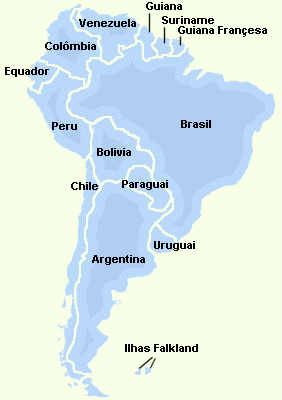
\includegraphics[scale=0.45]{img/southam_map_nocolor}}
\only<2>{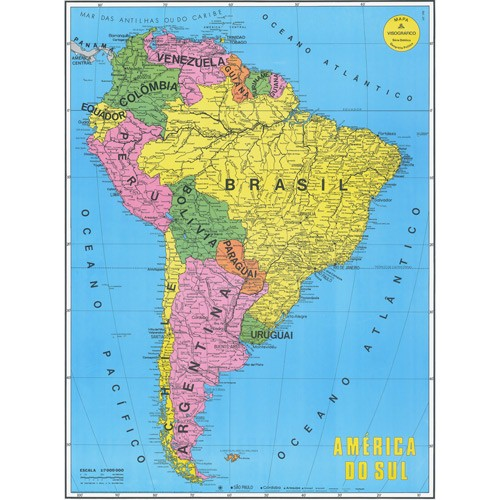
\includegraphics[scale=0.35]{img/southam_map_color}}
\end{column}
\begin{column}{0.55\textwidth}
\only<1>{\includegraphics[scale=0.2]{img/southam_nocolor.png}}
\only<2>{\includegraphics[scale=0.2]{img/southam_color.png}}
\begin{center}
{\footnotesize 1 -- Brasil, 11 -- Argentina}
\end{center}
\end{column}
\end{columns}

\end{frame}

\begin{frame}{Grafo: Definição}

\begin{block}{Informal}
Grafo G é formado:
\begin{itemize}
\item Conjunto finito de vértices $V$;
\item Relação simétrica $R$ em $V$ entre os pares de vértices;
\item O conjunto de pares simétricos $R$ é denotado por $E$.
\end{itemize}
\end{block}

\begin{block}{Formal}
$G = (V, E)$ \\
$\{v \in V : v \notin \emptyset\}$ \\
$\{ \{(u, v), (v, u)\} \in R : (u, v) \in E \land \{u, v\} \in V\}$ \\
\end{block}

\end{frame}

\begin{frame}{Representação simbólica: Exemplo}

$G = (V, E)$

$V = \{v_1, v_2, v_3, v_4, v_5\}$

$R = \{(v_1, v_2), (v_1, v_4), (v_2, v_1), (v_2, v_3), (v_2, v_4),
(v_3, v_2), (v_4, v_1), (v_4, v_2)\}$

$$ E = \{\{(v_1, v_2), (v_2, v_1)\}, \{(v_1, v_4), (v_4, v_1)\}, \{(v_2, v_3),$$  
$$(v_3, v_2)\}, \{(v_2, v_4), (v_4, v_2)\}\} $$

\end{frame}


\begin{frame}{Representação pictórica}

\begin{columns}
\begin{column}{0.6\textwidth}
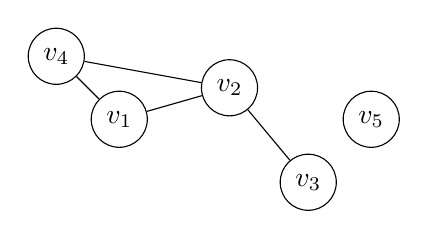
\begin{tikzpicture}[scale=0.8,mynode/.style=draw,circle]
\node[mynode] (v1) at (0,0) {$v_1$};
\node[mynode] (v2) at (1.75,0.5) {$v_2$};
\node[mynode] (v3) at (3,-1) {$v_3$};
\node[mynode] (v4) at (-1,1) {$v_4$};
\node[mynode] (v5) at (4,0) {$v_5$};
\draw (v1) -- (v2);
\draw (v1) -- (v4);
\draw (v2) -- (v4);
\draw (v2) -- (v3);
\draw (v5);
\end{tikzpicture}


\end{column}

\begin{column}{0.35\textwidth}
\scriptsize
\underline{\it Rótulos\/}\\
$v_1$ -- Brasil\\
$v_2$ -- Argentina\\
$v_3$ -- Chile \\
$v_4$ -- Paraguai \\
$v_5$ -- Equador
\end{column}

\end{columns}

\end{frame}

\begin{frame}{Matriz de adjacências}

\begin{columns}
\begin{column}{0.6\textwidth}
	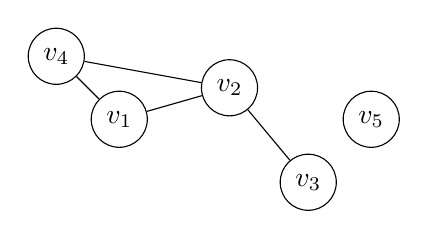
\begin{tikzpicture}[scale=0.8,mynode/.style=draw,circle]
\node[mynode] (v1) at (0,0) {$v_1$};
\node[mynode] (v2) at (1.75,0.5) {$v_2$};
\node[mynode] (v3) at (3,-1) {$v_3$};
\node[mynode] (v4) at (-1,1) {$v_4$};
\node[mynode] (v5) at (4,0) {$v_5$};
\draw (v1) -- (v2);
\draw (v1) -- (v4);
\draw (v2) -- (v4);
\draw (v2) -- (v3);
\draw (v5);
\end{tikzpicture}


\end{column}
\begin{column}{0.4\textwidth}
	$v_1  v_2  v_3  v_4  v_5$ \\
 	0  1  0  1  0 \\
 	1  0  1  1  0 \\
 	0  1  0  0  0 \\
 	1  1  0  0  0 \\
 	0  0  0  0  0
\end{column}
\end{columns}

\end{frame}


\begin{frame}{Representação de grafos usando lista ligada}

\begin{columns}
\begin{column}{0.375\textwidth}
	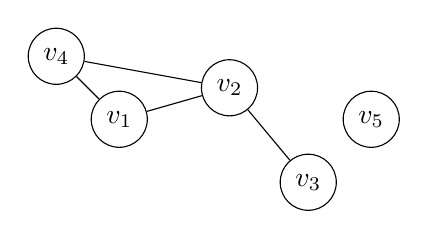
\begin{tikzpicture}[scale=0.8,mynode/.style=draw,circle]
\node[mynode] (v1) at (0,0) {$v_1$};
\node[mynode] (v2) at (1.75,0.5) {$v_2$};
\node[mynode] (v3) at (3,-1) {$v_3$};
\node[mynode] (v4) at (-1,1) {$v_4$};
\node[mynode] (v5) at (4,0) {$v_5$};
\draw (v1) -- (v2);
\draw (v1) -- (v4);
\draw (v2) -- (v4);
\draw (v2) -- (v3);
\draw (v5);
\end{tikzpicture}


\end{column}
\begin{column}{0.6\textwidth}
	\includegraphics[scale=0.275]{img/graph.png}
\end{column}
\end{columns}

\end{frame}


\begin{frame}{Grafos direcionados ou dígrafos: Definição}

\begin{block}{Informal}
Grafo direcionado ou dígrafo $G^\rightarrow$ é formado:
\begin{itemize}
\item Conjunto finito de vértices $V$;
\item Relação $R$ em $V$ entre os pares ordenados de arcos;
\item O conjunto de pares ordenados de arcos em $R$ é denotado por $E$.
\end{itemize}
\end{block}

\begin{block}{Formal}
$G^\rightarrow = (V, E)$ \\
$\{v \in V : v \notin \emptyset\}$ \\
$\{ (u, v) \in R : (u, v) \in E \land \{u, v\} \in V\}$ \\
\end{block}

\end{frame}


\begin{frame}{Dígrafo: exemplo}

\begin{block}{Representação simbólica}
\scriptsize
$G = (V, E)$

$V = \{v_1, v_2, v_3, v_4, v_5\}$
$R = \{(v_1, v_2), (v_2, v_3), (v_2, v_4), (v_4, v_1)\}$
$E  = \{(v_1, v_2), (v_4, v_1), (v_2, v_3), (v_2, v_4)\}$
     
\end{block}

\end{frame}

\begin{frame}{Dígrafo: Representação pictórica}

\begin{columns}
\begin{column}{0.6\textwidth}
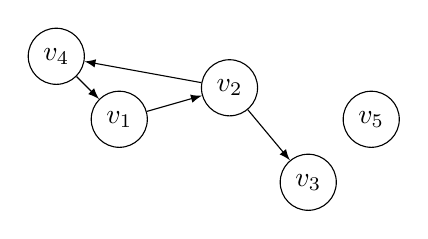
\begin{tikzpicture}[scale=0.8,mynode/.style=draw,circle,
                    goto/.style=->,>=latex]
\node[mynode] (v1) at (0,0) {$v_1$};
\node[mynode] (v2) at (1.75,0.5) {$v_2$};
\node[mynode] (v3) at (3,-1) {$v_3$};
\node[mynode] (v4) at (-1,1) {$v_4$};
\node[mynode] (v5) at (4,0) {$v_5$};
\draw[goto] (v1) -> (v2);
\draw[goto] (v4) -> (v1);
\draw[goto] (v2) -> (v4);
\draw[goto] (v2) -> (v3);
\draw[goto] (v5);
\end{tikzpicture}

\end{column}

\begin{column}{0.35\textwidth}
\scriptsize
\underline{\it Rótulos\/}\\
TODO
\end{column}

\end{columns}

\end{frame}

\begin{frame}{Representação usando matriz de adjacências}

\begin{columns}
\begin{column}{0.6\textwidth}
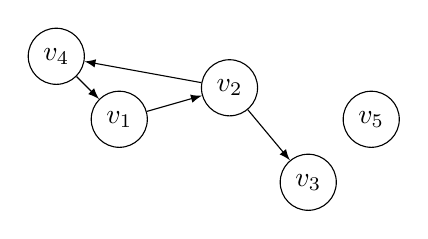
\begin{tikzpicture}[scale=0.8,mynode/.style=draw,circle,
                    goto/.style=->,>=latex]
\node[mynode] (v1) at (0,0) {$v_1$};
\node[mynode] (v2) at (1.75,0.5) {$v_2$};
\node[mynode] (v3) at (3,-1) {$v_3$};
\node[mynode] (v4) at (-1,1) {$v_4$};
\node[mynode] (v5) at (4,0) {$v_5$};
\draw[goto] (v1) -> (v2);
\draw[goto] (v4) -> (v1);
\draw[goto] (v2) -> (v4);
\draw[goto] (v2) -> (v3);
\draw[goto] (v5);
\end{tikzpicture}

\end{column}

\begin{column}{0.4\textwidth}
$ v_1  v_2  v_3  v_4  v_5$ \\
 0  1  0  0  0 \\
 0  0  0  0  0 \\
 0  1  0  0  0 \\
 1  1  0  0  0 \\
 0  0  0  0  0 \\
\end{column}
\end{columns}

\end{frame}

\begin{frame}{Representação usando lista ligada}

\begin{columns}
\begin{column}{0.4\textwidth}
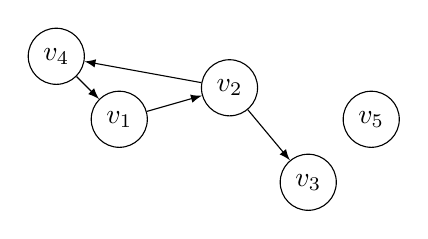
\begin{tikzpicture}[scale=0.8,mynode/.style=draw,circle,
                    goto/.style=->,>=latex]
\node[mynode] (v1) at (0,0) {$v_1$};
\node[mynode] (v2) at (1.75,0.5) {$v_2$};
\node[mynode] (v3) at (3,-1) {$v_3$};
\node[mynode] (v4) at (-1,1) {$v_4$};
\node[mynode] (v5) at (4,0) {$v_5$};
\draw[goto] (v1) -> (v2);
\draw[goto] (v4) -> (v1);
\draw[goto] (v2) -> (v4);
\draw[goto] (v2) -> (v3);
\draw[goto] (v5);
\end{tikzpicture}

\end{column}
\begin{column}{0.6\textwidth}
 \includegraphics[scale=0.35]{img/digraph.png}
\end{column}
\end{columns}

\end{frame}

\end{document}
